\chapter{開発プロセス}

\section{OJL}

TLVは,OJL(On the Job Learning)の開発テーマとして開発された.
OJLとは,企業で行われているソフトウェア開発プロジェクトを教材とする実践教育であり,製品レベルの実システムの開発を通じて創造的な思考力を身につけるとともに,単なる例題にとどまらない現実の開発作業を担うことにより,納期,予算といった実社会の制約を踏まえたソフトウェア開発の実際について学ぶことを目的としている.

TLVはプロジェクトベースで開発が行われ,企業出身者2名と教員1名がプロジェクトマネージャを務め,学生3名(筆者含む)と企業出身者2名が開発実務を行った.
進捗の報告は,週に1度のミーティングと週報の提出により行った.

\subsection{フェーズ分割}

単年度でTLVを開発するにあたり,全体を3フェーズに分割した.
各々のフェーズの内容は次の通りである.

\subsubsection{フェーズ1}

\begin{description}
\item[期間] \mbox{} \\
2008年5月~同年8月(約3ヶ月)

\item[目的・目標] \mbox{} \\
プロトタイプの実装を行い,そのプロセスと成果物から,GUIの評価や要求の再抽出,アプリケーションドメイン分析を通じた設計方法の探索を行う.

\item[実装内容] \mbox{} \\
機能を限定して実装を行う.

トレースログの対象をTOPPERS/ASPカーネルに絞り,可視化表示項目もタスクの状態遷移のみとする.

標準形式トレースログへの変換や,可視化ルールの適用による可視化表示は行わない.

\item[実施結果] \mbox{} \\
実装成果物の総行数は約9000行(有効行数5000行)であった.

開発関係者4名とRTOS開発者および利用者の7名に成果物を利用してもらい意見を収集した.
その結果,ユーザインタフェース,追加の機能要求,可視化表現項目について意見が得られた.

実装中心の開発プロセスになってしまい,チーム開発がうまく機能しなかった.

\end{description}

\subsubsection{フェーズ2}

\begin{description}
\item[期間] \mbox{} \\
2008年9月~2009年1月(約5ヶ月)

\item[目的・目標] \mbox{} \\
標準形式トレースログの策定,可視化ルールの策定.
標準形式トレースログへの変換,可視化ルールファイルによる可視化表示の外部プラグイン化の実装.
ユースケース駆動アジャイル開発の導入.

\item[実装内容] \mbox{} \\
主要機能である,標準形式トレースログへの変換,可視化ルールファイルによる可視化表示の外部プラグイン化を実装する.
また,フェーズ1にて再定義された機能要求を可能な限り実装する.

\item[実施結果] \mbox{} \\
実装成果物の総行数は約18500行(有効行数10300行)であった.

標準形式トレースログ,可視化ルールファイル,またリソースファイル,リソースヘッダファイルの形式を本論文で述べたとおり定義した.

また,本論文で示したとおり,標準形式トレースログへの変換と可視化ルールファイルによる可視化表現項目の追加を実現できた.

ユースケース駆動アジャイル開発により,ユースケース毎にイテレーションを繰り返し実施し開発を行った.
結果,36個中27個のユースケースについて実装が完了した.

\end{description}

\subsubsection{フェーズ3}

\begin{description}
\item[期間] \mbox{} \\
2008年2月~2009年3月(約1ヶ月)

\item[目的・目標] \mbox{} \\
TLVで読み込めるトレースログ形式を増やす.
可視化表現項目を増やす.

\item[実装内容] \mbox{} \\
フェーズ2の成果を元に,変換ルールファイルを追加・変更し対応するトレースログの形式を増やす.また,可視化ルールファイルを追加・変更し可視化表現項目の充実を図る.

\item[実施結果] \mbox{} \\
未実施である.

\end{description}


\section{ユースケース駆動アジャイルソフトウェア開発}
\label{usecaseAgile}

フェーズ2において,TLVの開発は,ユースケース駆動アジャイルソフトウェア開発という手法を用いて行われた.

アジャイルソフトウェア開発では,反復(イテレーション)と呼ばれる短い期間を単位に反復して開発を行い,計画ではなく状況において適応的に対応することを重視してソフトウェア開発を行う.
1つのイテレーション内では1つの機能に対して設計,実装,テスト,文書化といった工程を完結して行う.
TLVの開発ではユースケースを機能の単位にイテレーションを反復して実施した.
図\ref{fig:agile}にユースケース駆動アジャイルソフトウェア開発の例を示す.

\begin{figure}[t]
\begin{center}
\includegraphics[scale=0.75]{img/agile.eps}
\caption{ユースケース駆動アジャイルソフトウェア開発}
\label{fig:agile}
\end{center}
\end{figure}

はじめに外部設計としてユースケース図,ユースケース内のクラス図,シーケンス図を作成する.
次に,クラス単位で内部設計,単体テスト,実装を行う.
内部設計では,クラス図で定義したクラスに関してインタフェースのみを記述したスケルトンを作成し,コメントとして内部設計を記述する.
単体テストは,メソッド単位のユニットテストとし,統合開発環境に付属するユニットテストフレームワークを用いて実装,実施する.
単体テストの実装はテストケースの記述であり,ユニットテストフレームワークが出力するテストコードのスケルトンに必要な情報を記述することで行う.
単体テストの実装が終わったらクラスの実装を行う.
クラスの実装は,単体テストを実施しながら,テスト項目のをすべてを成功するかどうか試しながら行う.
1つのクラスの実装が終わればユースケース内の次のクラスの内部設計に移る.

このようにしてユースケース内のクラスをすべて実装したら,ユースケース内のクラスを結合してユースケースとして駆動する形に実装する.
この際も,テストケースの実装を先に行ってから実装を開始する.
結合テストのテスト項目のをすべてを成功したら,1つのイテレーションの完了であり,次のユースケースの外部設計を開始する.

本節では,TLVの開発において,ユースケース駆動アジャイルソフトウェア開発の各工程で実践した内容について詳述する.

\subsection{プロジェクト管理}

フェーズ2のはじめの作業として,フェーズ1で行った評価の結果と,フェーズ2の実施概要について,プロジェクト計画書として文書化した.

次に,フェーズ2で実装するTLVの機能を,要求仕様書として文書化した.
また,機能をユースケースを単位に定義し,ユースケース図を作成した.
図\ref{fig:usecase}にTLVのユースケース図を示す.

\begin{figure}[t]
\begin{center}
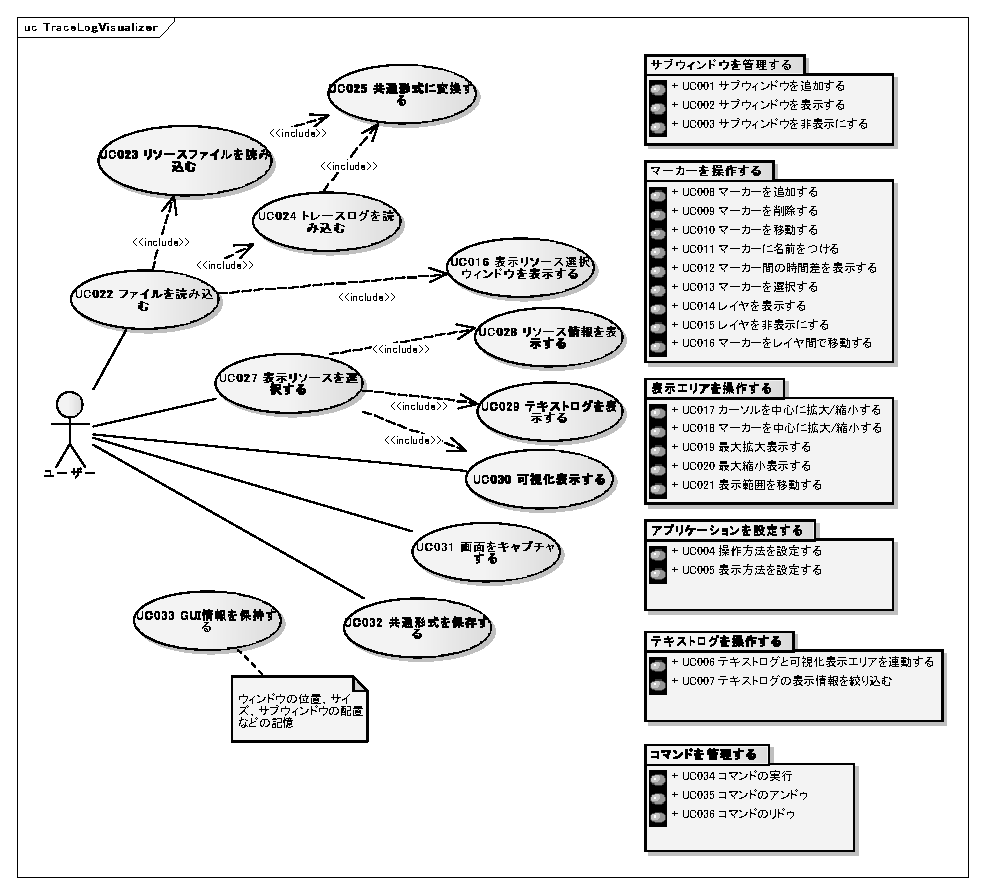
\includegraphics[scale=0.75]{img/usecase.eps}
\caption{TLVのユースケース図}
\label{fig:usecase}
\end{center}
\end{figure}

TLVの機能をユースケースを単位に定義した結果,全ユースケース数は36個であった.
これらのユースケースを工程毎に分けた進捗表を作成し,これを用いて進捗管理を行い,複数のメンバーで工程の分担,作業項目の同期を行った.

\subsection{設計}

図\ref{fig:agile}に示すとおり,外部設計としては,ユースケース内のクラスについて,クラス図を,クラス間の連携の流れをシーケンス図として作成することで行う.
図\ref{fig:class}に作成したクラス図の例を示す.
また,図\ref{fig:sequence}に作成したシーケンス図の例を示す.

\begin{figure}[t]
\begin{center}
\includegraphics[width=13cm]{img/class.eps}
\caption{TLVの外部設計で作成したクラス図の例}
\label{fig:class}
\end{center}
\end{figure}

\begin{figure}[t]
\begin{center}
\includegraphics[width=13cm]{img/sequence.eps}
\caption{TLVの外部設計で作成したシーケンス図の例}
\label{fig:sequence}
\end{center}
\end{figure}

内部設計は文書化せずに,ソースコードのコメントを記述することで行った.
外部設計で作成したクラス図を元に,インタフェースのみを記述したクラスを記述し,メソッドのコメントとして,引数,返値の説明,どのような内部実装を行うべきかの説明を記述する.

\subsection{テスト}

TLVのテストは,統合開発環境に付属するユニットテストフレームワークを用いて実装,実施した.
ユニットテストフレームワークは,クラスのメソッドの定義を元に,テストケースのスケルトンを自動生成する仕組みを搭載しており,テスト工程作業の大幅な省力化を図ることができる.
スケルトンは,引数の組み合わせと期待値を開発者が入力するように生成されており,これらを入力する作業が実質的なテストケースの実装作業となる.

ユニットテストの単位はメソッドだが,単純なアクセサメソッドはテストの対象外とした.
その結果,491メソッドがユニットテストの対象となった.

\subsection{実装}

TLVの実装言語は,C$\sharp$ 3.0である.
統合開発環境として Microsoft Visual Studio 2008 Professional Edition を用いた.
TLVの実行には .NET Framework 3.5 が必要である.

実装はクラス単位で行い,ユニットテストが全部成功することを目標に行う.
その際,テストの実施とクラスの実装は反復して行う.
テスト結果は記録されるため,文書化する必要がなく,素早くデバッグを行うことができる.

TLVのソースコードメトリクスを表\ref{sourceMetrics}に示す.

\begin{table}[htb]
\begin{center}
\caption{TLVのソースコードメトリクス}
\label{sourceMetrics}
\begin{tabular}{l|l}
\hline
総行数              & 18497 \\
ファイル平均行数    & 94.38 \\
有効な行数          & 10332 \\
コメント行数        & 1432 \\
空行                & 2224 \\
その他の行数(中括弧など) & 4509 \\
ファイル数          & 196 \\
クラス数            & 186 \\
構造体数            & 0 \\
インタフェース数    & 22 \\
列挙体              & 15 \\
デリゲート          & 2 \\
\hline
\end{tabular}
\end{center}
\end{table}

